\section{Testing and Observations}

\subsection{Microphone/ADC}
Regarding microphone data, there were two aspects of this component that needed to be tested. The first was the polling rate and making sure that we were in fact sampling at the correct frequency when starting DMA. Due to our sampling rate being 10kHz, and to our buffer having 10000 entries, our total time between HAL\_ADC\_Start\_DMA and the callback of the HAL\_ConvCmplCallback needed to be exactly one second. This was confirmed via the blinking red LED on board which indicates that the ADC is sampling, and more accurately with the Keil timer in the debugger to accurately time the period between the two functions mentioned above. The second aspect that needed to be tested was the actual microphone data as see if the values recorded can be trusted and used. Our first test was to connect the ADC input pin to the 5v pin of the Discovery board. The values expected to be read would be the maximum 12 bit value that our ADC could convert, $2^{12} = 4095$. Once confirmed that the ADC value would change we connected the microphone and captured some test measurements of 1 second samples of sound. The following figure shows the captured sample of the spoken number .

\begin{figure}[h]
	\caption{Capture 10kHz sample of the spoken digit seven}\label{fig:speechseven}
	\begin{center}
		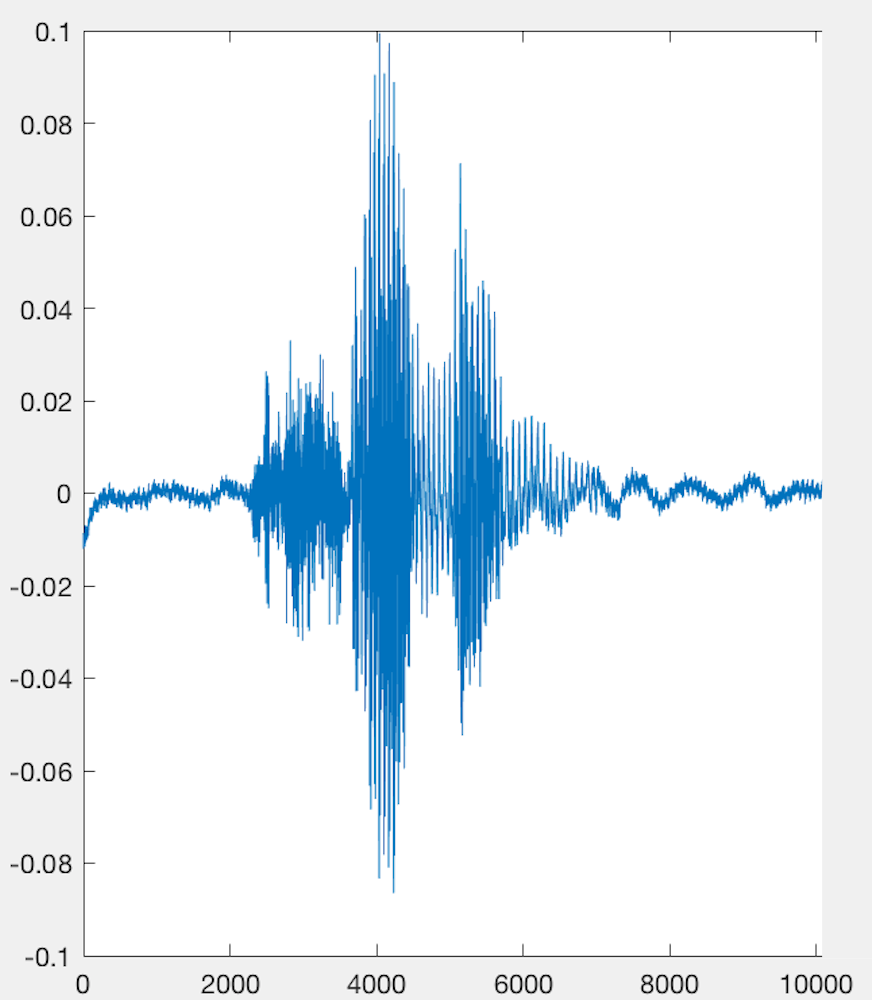
\includegraphics[scale=0.5]{speech_seven}
	\end{center}
\end{figure}

With testing at different sampling rates, we decided that 10kHz was the lowest we would be willing to go so that the speech API on the hosted web page end of the pipeline would be able to accurately recognize what the spoken digit is. We also noted that most captured samples varied greatly in the amount of noise they produced, and were we to have more time, a digital or analog low pass filter prior to running our speech through the speech API would be needed to increase the accuracy of our number recognition.


\subsection{Accelerometer}
Our accelerometer component was tested in a similar way compared to the microphone. The first test we ran was to see if our watch variables in Keil would be updated at the right frequency and display reasonable values for pitch and roll when our board is flat on a surface. As seen in Figure 7, or final test to confirm if our accelerometer data was really valid was to display it on our hosted web page. The resulting data is due to the user rotating the discovery board and then setting it down. Because the board was propped up on one end to allow for easier threshold detecting when tapping and double tapping, the resting pitch is 0 but the roll is negative due to the board's angle. With our data making sense, we decided that having LEDs display the intermediate state of the FSM's First Tap state (Seen in Figure 4) would give good user feedback for how fast they needed to double tap and if the board had even detected their first tap. With our board propped on a surface with more give and bounce, coupled with the LED user feedback of the tap detection, our accelerometer was working most of the time and with rare detection misses.

\subsection{UART}
UART transmission between the nucleo and discovery was simple and easy to test. With one of the devices waiting on a UART\_Receive with a MAX\_Timeout delay and the other transmitting we would be able to watch the receiving buffer fill up when the interrupt was triggered from having received the set amounts of bits from the transmitter. Through our numerous tests, we noticed that data transmission was very reliable as long as the receiving end managed to enter their UART\_Receive state before the sender ever starts transmitting data. 

\subsection{BLE}
asd

\subsection{Android Application}
The android testing required us to be able to connect to the nucleo and receive the microphone and accelerometer GATT characteristics when connecting at the start. This was made easier with Android Device Bridge (ADB) which let us monitor the android logs as they happened in real time. We were able to see when the connection was being established through the UI of the application, but being able to see the BLE packets coming in with their corresponding characteristics let us know exactly when our application was receiving data. 

\subsection{Web Server}
Testing this last stage of our project was challenging as our microphone and accelerometer data had to make it all the way to the end of the pipeline. Due to this stage's dependencies on prior components not only working individually, but also working as a whole, we created testing functions that would test the server's ability to accept and process data. This was done with the functions in the api\_test.py file where the function 
test\_with\_live\_recording would replicate the same sampling as our ADC and pass it through to the speech API for processing and the result is subsequently printed. For testing in our full pipeline we ended up tracking the server logs (similar to testing with ADB) as the android connection was being established and data was being transmitted. As a final check prior to the data being either graphed or processed in the speech API, we compared the data transmitted at this point with our known sample points in our buffers on the nucleo and discovery to make sure the data was consistent. As discussed in the microphone testing section, we noticed that due to the low quality audio playback of 8kHz sampled audio, and the fact that the API was trained on speech at higher sampling rates, we decided to use a bigger buffer to store the speech on our hardware for the increased performance of our speech recognition in the cloud.

\subsection{Entire System}
Talk about overall functionality of the pipeline and what worked.